\documentclass{exam}
\usepackage[utf8]{inputenc}
\usepackage{lmodern}
\usepackage{microtype}

% \usepackage[parfill]{parskip}
\usepackage[dvipsnames]{xcolor}
\usepackage{amsmath}
\usepackage{amsfonts}
\usepackage{amsthm}
\usepackage{siunitx}
\DeclareSIUnit\year{yr}
\DeclareSIUnit\foot{ft}
\DeclareSIUnit\litre{\liter}

\usepackage{skull}

\usepackage{pgfplots}
\usepgfplotslibrary{polar}
\pgfplotsset{compat=1.11}
\usepgfplotslibrary{statistics}
\usepackage{graphicx}
\usepackage{sidecap}
\sidecaptionvpos{figure}{c}
\usepackage{float}
\usepackage{gensymb}
\usepackage{tkz-euclide}
\usetkzobj{all}
\usepackage{commath}
\usepackage{hyperref}
\usepackage{enumitem}
\usepackage{wasysym}
\usepackage{multicol}
\usepackage{mathtools}
\usepackage{tcolorbox}
\usepackage{tabularx}
\usepackage[version=4]{mhchem}
\usepackage{changepage}
\usepackage{listings}
\lstset{basicstyle=\ttfamily\linespread{0.8}\small}

\renewcommand*{\thefootnote}{\fnsymbol{footnote}}

\newtheorem*{thm}{Theorem}
\newtheorem*{iden}{Identity}
\newtheorem*{lemma}{Lemma}
\newtheorem{obs}{Observation}
\theoremstyle{definition}
\newtheorem*{defn}{Definition}
\newtheorem*{ex}{Example}
\newtheorem{con}{Construction}
\newtheorem*{alg}{Algorithm}

\newtheoremstyle{break}
  {\topsep}{\topsep}%
  {\itshape}{}%
  {\bfseries}{}%
  {\newline}{}%
\theoremstyle{break}
\newtheorem*{bthm}{Theorem}

% russian integral
\usepackage{scalerel}
\DeclareMathOperator*{\rint}{\scalerel*{\rotatebox{17}{$\!\int\!$}}{\int}}

% \DeclareMathOperator*{\rint}{\int}

\pgfplotsset{vasymptote/.style={
    before end axis/.append code={
        \draw[densely dashed] ({rel axis cs:0,0} -| {axis cs:#1,0})
        -- ({rel axis cs:0,1} -| {axis cs:#1,0});
    }
}}

% \pointsinrightmargin
\boxedpoints
\pointname{}

\newcommand{\questioA}{\question[\texttt{\textbf{\color{Cerulean} A}}]}
\newcommand{\questioM}{\question[\texttt{\textbf{\color{PineGreen} M}}]}
\newcommand{\questioE}{\question[\texttt{\textbf{\color{WildStrawberry} E}}]}
\newcommand{\questioS}{\question[\texttt{\textbf{\color{Goldenrod} S}}]}
\newcommand{\questioO}{\question[\texttt{\textbf{\color{BurntOrange} O}}]}

\newcommand{\parA}{\part[\texttt{\textbf{\color{Cerulean} A}}]}
\newcommand{\parM}{\part[\texttt{\textbf{\color{PineGreen} M}}]}
\newcommand{\parE}{\part[\texttt{\textbf{\color{WildStrawberry} E}}]}
\newcommand{\parS}{\part[\texttt{\textbf{\color{Goldenrod} S}}]}
\newcommand{\parO}{\part[\texttt{\textbf{\color{BurntOrange} O}}]}

\newcommand{\subparA}{\subpart[\texttt{\textbf{\color{Cerulean} A}}]}
\newcommand{\subparM}{\subpart[\texttt{\textbf{\color{PineGreen} M}}]}
\newcommand{\subparE}{\subpart[\texttt{\textbf{\color{WildStrawberry} E}}]}
\newcommand{\subparS}{\subpart[\texttt{\textbf{\color{Goldenrod} S}}]}
\newcommand{\subparO}{\subpart[\texttt{\textbf{\color{BurntOrange} O}}]}

\newcommand{\mainHeader}[2]{\section*{NCEA Level 2 Mathematics\\#1. #2}}
\newcommand{\mainHeaderHw}[2]{\section*{NCEA Level 2 Mathematics (Homework)\\#1. #2}}
\newcommand{\seealso}[1]{\begin{center}\emph{See also #1.}\end{center}}
\newcommand{\drills}[1]{\begin{center}\emph{Drill problems: #1.}\end{center}}
\newcommand{\basedon}[1]{\begin{center}\emph{Notes largely based on #1.}\end{center}}

\begin{document}

\mainHeaderDiff{8}{Optimisation}
Recall from Level 2 that a \textit{local maximum} of a function $ f $ is some point $ (x, f(x)) $
such that, for a sufficiently small interval $ I $ around $ x $, for all $ y \in I $ $ f(y) \leq f(x) $;
a \textit{local minimum} is defined in a similar way (see exercises).

\begin{ex}
  The function $ x \mapsto x^2 $ has a local minimum at $ (0, 0) $.
\end{ex}
\begin{ex}
  The function $ x \mapsto 2x^3 + 15x^2 + 36x + 2 $ has a local maximum at $ (-3, -25) $ and a local minimum at $ (-2, -26) $.
\end{ex}
\begin{ex}
  The function $ x \mapsto \sin x $ has a local maximum at $ (2n\pi + \frac{\pi}{2}, 1) $ for every $ n \in \mathbb{Z} $, and
  a local minimum at $ (2n\pi - \frac{\pi}{2}, 1) $ for every $ n \in \mathbb{Z} $.
\end{ex}

Local extrema are also sometimes called \textit{relative extrema}.

It is possible to prove that if $ f $ is defined around some value $ x $, if $ f $ has a relative extremum at $ (x, f(x)) $, and
if $ f' $ is defined at $ x $, then $ f'(x) = 0 $. Because of this, we define a \textit{critical point}
of a function $ f $ to be some value $ x $ such that either $ f'(x) = 0 $, or $ f'(x) $ is undefined. In the first case, we also
call the value a \textit{stationary point}.

\textbf{All local extrema occur at critical points, but not all critical points occur at extrema.}

\begin{ex}
  The function $ x \mapsto 2x^3 + 15x^2 + 36x + 2 $ above has critical points $ x = -2 $ and $ x = -3 $. Both of
  these are local extrema.
\end{ex}

\begin{ex}
  The function $ x \mapsto x^3 $ above has a critical point at $ x = 0 $, but does not have a local extrema there.
\end{ex}

\begin{ex}
  The function $ x \mapsto \frac{1}{x} $ \textit{does not} have a critical point at $ x = 0 $, \textbf{because it is not defined there}.
\end{ex}

We can use the first derivative to classify extrema as either maxima or minima.
\subsubsection*{The First Derivative Test}
\begin{enumerate}
  \item Determine all critical points of $ f $.
  \item Determine the sign of $ f'(x) $ to the left and right of each critical point $ x_0 $:
    \begin{itemize}
      \item If $ f'(x) $ changes from positive to negative as we move from left to right across $ x_0 $, then $ f(x) $ has a local maximum at $ x_0 $.
      \item If $ f'(x) $ changes from negative to positive as we move from left to right across $ x_0 $, then $ f(x) $ has a local minimum at $ x_0 $.
      \item If $ f'(x) $ does not change sign across $ x_0 $, then $ f(x) $ does not have a relative extremum at $ x_0 $ (e.g. $ y = x^3 $).
    \end{itemize}
\end{enumerate}

Recall last week's material; using the second derivative, we can come up with a second test:
\subsubsection*{The Second Derivative Test}
\begin{enumerate}
  \item Compute $ f'(x) $ and $ f''(x) $.
  \item Find all the stationary points of $ f $ by finding all the points $ x_0 $ such that $ f'(x_0) = 0 $.
  \item Determine the sign of $ f''(x) $ for each stationary point $ x_0 $:
    \begin{itemize}
      \item If $ f''(x_0) < 0 $, then $ f(x) $ has a relative maximum at $ x_0 $.
      \item If $ f''(x_0) > 0 $, then $ f(x) $ has a relative minimum at $ x_0 $.
      \item If $ f''(x_0) = 0 $, then $ f(x) $ could have a relative maximum, a relative minimum, or neither.
    \end{itemize}
\end{enumerate}

\begin{ex}
  Find and classify the critical points of $ y = x^3 - 3x^2 + 6 $.

  \textit{Solution.} We have $ \od{y}{x} = 3x^2 - 6x $ and $ \od[2]{y}{x} = 6x - 6 $. Hence
                     the critical points are $ x = 0 $ and $ x = 2 $. At the former point, $ \od[2]{y}{x} < 0 $,
                     and so the point is a maximum; at the latter point, $ \od[2]{y}{x} > 0 $ and so the point is
                     a minimum.
\end{ex}

\begin{ex}
  Find two numbers whose difference is 100 and whose product is a minimum.

  \textit{Solution.} Let the two numbers be $ x $ and $ x + 100 $. We wish to minimise $ y = x(x + 100) $;
  clearly $ y' = 2x + 100 $, and so $ x = -50 $ is a critical point. To the left of $ x = -50 $, the derivative
  is negative; to the right, the derivative is positive. Hence $ x = -50 $ is indeed a minimum. The two required
  numbers are therefore -50 and 50.
\end{ex}

\begin{ex}
  Find and classify the critical points of $ y = (x - 1)^2 + \ln x $.

  \textit{Solution.} The derivative is $ y' = 2x - 2 + \frac{1}{x} $. We therefore have one critical
  point at $ x = 0 $ (where $ y' $ is undefined); this is an asymptote.
  Setting $ y' = 0 $, we have $ 0 = 2x - 2 + \frac{1}{x} = 2x^2 - 2x + 1 $ which has no real roots. Hence $ x = 0 $ is
  the only critical point, and the curve has no local extrema.
\end{ex}

\begin{ex}
  A rectangular plot of land is to be fenced using two varieties of fence. Two opposite sides will
  use fences selling for \$3 per metre, while the other two sides will use cheaper fence selling for \$2 per metre.
  Given that the total budget is \$1200, what is the greatest area of land which can be fenced?

  \textit{Solution.} Let $ x $ be the length of one of the expensive sides; then the length of one of the cheaper
                    sides is $ \frac{1}{2}(1200 - 3x) $, and the total area is $ A = \frac{1}{2} x (1200 - 3x) = \frac{1}{2}(1200x - 3x^2) $.
                    Hence $ \od{A}{x} = 600 - 3x $. We wish to find the maximum area, so set $ \od{A}{x} = 0 $; hence $ 3x = 600 $ and $ x = 200 $.
                    Note that the second derivative is always negative, so this stationary point must be a maximum as required. The length
                    of the other side will be $ \frac{1}{2}(1200 - 600) = 300 $, and so the maximum area is $ 300 \times 200 = 60000 $ square metres.
\end{ex}

\subsection*{Questions}
\begin{questions}
  \questioA Write down a definition of a local minimum similar to that given for a maximum.
  \questioA Show that $ f(x) = x^4 $ has $ f''(0) = 0 $ but not a point of inflection at $ x = 0 $ (in fact, it has a minimum at that point).
  \questioA Describe the advantages and disadvantages of the first and second derivative tests for local extrema.
  \questioM Describe the local extrema, concavity, and points of inflection of the function $ f(x) = x^4 - 4x^3 $.
  \questioA Consider the following graph:
            \begin{center}
              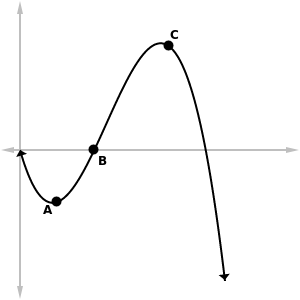
\includegraphics[width=0.3\textwidth]{curvature}
            \end{center}
            Find the signs of $ \od{y}{x} $ and $ \od[2]{y}{x} $ at the three points $ A $, $ B $, and $ C $.
  \questioA Without using calculus, find the extreme value(s) of $ y = 3x^2 - 258x + 5598 $.
  \questioM Find all the local extrema of the following curves in the given intervals, and classify them as maxima, minima, or neither.
    \begin{parts}
      \part $ f(x) = \sin x - \cos x $ on the interval $ 0 < x < \pi $
      \part $ g(x) = x^3 - x^2 + x - 1 $ on the interval $ -\infty < x < \infty $
    \end{parts}
  \questioM The sum of two positive numbers $ x $ and $ y $ is 16. Find the smallest possible value for $ S = x^2 + y^2 $.
  \questioM A box with an open top is to be constructed from a square piece of cardboard with a side length of \SI{3}{\metre}
            by cutting out a square from each of the four corners and bending up the sides. Find the dimensions of the resultant
            box of maximum volume.
  \questioM Find the dimensions of a rectangle with area \SI{1000}{\metre\squared} such that the perimeter is minimised.
  \questioE A large orange rectangle is to be drawn with one corner sitting on the origin and the opposite corner lying on
            the curve $ y = 0.2(x - 10)^2 $. What is the maximum possible area of the rectangle?
            \begin{center}
              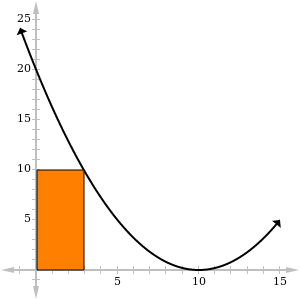
\includegraphics[width=0.3\textwidth]{paramax}
            \end{center}
  \questioM A window consisting of a rectangle topped with a semicircle is to have a fixed perimeter $ p $. Find the radius
            of the semicircle in terms of $ p $ if the total area is to be maximised.
  \questioE A thin wire of length $ L $ is cut in two and the resulting lengths are bent to make a square and an equilateral triangle. Where
            should the wire be cut to make the total area of the shapes (a) a maximum and (b) a minimum?
  \questioE Find the point on the line $ y = 2x + 3 $ closest to the origin.
  \questioE Find the point on the curve $ y = \sqrt{x} $ closest to $ (3, 0) $.
  \questioM The rate in which photosynthesis takes place for a species of phytoplankton is modeled by the function
            \begin{displaymath}
              P = \frac{100I}{I^2 + I + 4}.
            \end{displaymath}
            For which light intensity $ I $ is $ P $ a maximum?
  \questioE By finding the $ x$- and $ y$- intercepts, the asymptotes, the critical points, the
            intervals of increase and decrease, the intervals of concavity, and any other important
            points, sketch the following functions (199):
    \begin{parts}
      \part $ f(x) = \frac{x^2}{4 - x^2} $
      \part $ f(x) = \frac{4x}{x^2 + 1} $ [\textit{Hint: consider what happens to $ f(x) $ as $ x \to \pm\infty $.}]
      \part $ f(x) = \frac{x^2 - 4x + 5}{x - 2} = x - 2 + \frac{1}{x - 2} $ [\textit{Hint: consider what happens to $ f(x) - (x - 2) $ as $ x \to \pm\infty $.}]
    \end{parts}
  \questioE A cone with height $ h $ is inscribed in a larger cone of height $ H $ such that the vertex of the small cone
            is at the centre of the base of the larger cone. Show that the maximum volume of the smaller cone occurs when $ h = \frac{1}{3} H $.
  \questioE Let $ v_1 $ be the velocity of light in air and $ v_2 $ be the velocity of light in water. A ray of light will travel from a point $ A $
            in the air to a point $ B $ in the water by a path $ ACB $ that minimises the time taken. Show that
            \begin{displaymath}
              \frac{\sin \theta_1}{\sin \theta_2} = \frac{v_1}{v_2}
            \end{displaymath}
            where $ \theta_1 $ is the angle of incidence and $ \theta_2 $ is the angle of refraction.
            \begin{center}
              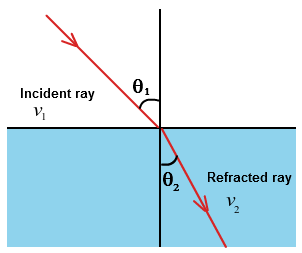
\includegraphics[width=0.3\textwidth]{snell}
            \end{center}
  \questioE Show that the polynomial $ p(x) = 10x^3 + x^2 + x - 34 $ has exactly one real zero.
  \questioE A rain gutter is to be constructed from a metal sheet of width \SI{30}{\centi\metre} by bending up
            one third of the sheet on each side by an angle $ \theta $. What angle should be chosen in order to
            obtain the maximum possible volume?
  \questioE A steel pipe is carried around a right-angled corner from a hallway \SI{3}{\metre} wide into a hallway \SI{2}{\metre}
            wide. What is the length of the longest pipe that can be carried horizontally around the corner? [\textit{Hint: this is actually
            a minimisation problem, despite the wording.}]
  \questioE Find and classify the critical points of $ h(x) = x^4 + x^3 + cx^2 $.
  \questioS Show that $ \frac{x^2 + 1}{x} \geq 2 $; hence (or otherwise) show that $ \frac{(x^2 + 1)(y^2 + 1)(z^2 + 1)}{xyz} \geq 8 $.
  \questioS Scholarship 2013: Prince Ruperts drops are made by dropping molten glass into cold water. A mathematical model for a drop
            as a volume of revolution uses $ y = \sqrt{\phi (e^{-x} - e^{-2x})} $ for $ x \geq 0 $, where $ \phi $ is the golden
            ratio $ \phi = \frac{1 + \sqrt{5}}{2} $.
    \begin{parts}
      \part Where is the modelled drop widest, and how wide is it there?
      \part The drop changes shape at a point $ B $, where the concavity of the function is zero. Use
            \begin{displaymath}
              \od[2]{y}{x} = \sqrt{\phi} \frac{e^{2x} - 6e^x + 4}{y^2 e^{4x}}
            \end{displaymath}
            to find the exact $ x$-ordinate of $ B $.
    \end{parts}

\end{questions}
\end{document}
